\documentclass[fleqn]{jbook}
\usepackage{physpub}

\begin{document}
\begin{question}{教育 物理}{}

%第1問
\begin{subquestions}
\SubQuestion
ロケットを垂直上方に打ち上げて、地球の重力圏を脱したい。時刻$t$におけるロケットの高さ、速度および質量をそれぞれ$h(t),\ v(t)=\frac{\d{h}}{\d{t}},\ M(t)$、ロケットから噴射されるガスの、ロケットに対する相対速度を$u$とする。重力加速度を$g=9.8$ m/s$^2$、地球の半径を$R=6370$ kmとして、以下に答えよ。なお、相対速度$u$は一定であるとし、空気抵抗は無視せよ。

\begin{subsubquestions}
\SubSubQuestion
地球の重力圏を脱出するためには噴射が終わったときの速度がある値(脱出速度:$v_{\text{esc}}$)を越えている必要がある。噴射終了時の高度は$R$に比べて十分小さいとして$v_{\text{esc}}$を求めよ。

\SubSubQuestion
ロケットの運動方程式は、
\[
M\frac{\d{v}}{\d{t}} = -u\frac{\d{M}}{\d{t}} - Mg
\]
で与えられる。この式を導け。

\SubSubQuestion
燃料の噴射時間を$\Delta t$とし、噴射開始時および噴射終了時の全質量をそれぞれ、$M_i=M(t_0),\ M_f=M(t_0+\Delta t)$とおくとき、この間の速度変化$\Delta v=v(t_0+\Delta t)-v(t_0)$を求めよ。また、噴射時間内の速度変化$\Delta v$を増やすにはどうしたらよいかを述べよ。

\SubSubQuestion
簡単のため、ロケットの加速度は一定であるとし、$\frac{\d{v}}{\d{t}}=ng$とおく。ここに、加速度係数$n$は、乗組員や機内の装置に支障が生じないように選ばれた定数である。噴射開始時の質量$M_i$と噴射終了時の質量$M_f$の差がすべて燃料であるとして、燃料噴射時間$\Delta t$、噴射による速度変化$\Delta v$、および高度変化$\Delta h$を求めよ。

\SubSubQuestion
燃料の燃焼温度を$T$ Kとするとき、燃料ガスの噴射速度$u$は、燃料の分子がこの温度の下で持つ平均の運動エネルギーから決まる平均速度を超えられない。燃料分子の質量を$m$、ボルツマン定数を$k$として、燃料分子の平均速度$u_0$をあらわせ。また、$u=u_0$が実現できたとして、燃料ガスの噴射速度を大きくするには、どうしたらよいかを述べ、最良の燃料として何を選んだらよいかを言え。

\SubSubQuestion
燃焼温度を$T=2000$ K、$k=1.4\times 10^{-23}$ J/K、陽子の質量$m_p$を$1.7\times 10^{-27}$ kgで与えられるとき、設問(v)で選んだ燃料から期待される最高噴射速度を求めよ。

\SubSubQuestion
実際のロケットでは、構造上、噴射開始時および噴射終了時の全質量の比$\frac{M_i}{M_f}$は、高々4程度にしかできない。燃料ガスの噴射速度を$u=3$ km/s、加速度係数を$n=4$として、期待される最終速度を求め、脱出速度と比較せよ。この結果と設問(v)と(vi)の結果から、脱出速度を得るためにどういう工夫をしたらよいかを論ぜよ。ただし、$\ln 2=\log_e 2=0.7$とおけ。

\end{subsubquestions}

%第2問
\SubQuestion
半径aの円形断面を持つ無限に長い直線導線がある。電流が流れていないとき、導線内の電荷分布は一様で、正電荷密度は$\rho_+=\rho_0$、伝導電子による負電荷密度は$-\rho_-=-\rho_0$であるが、電流を流すと、負電荷密度$-\rho_-$には$-\rho_0$からのずれが生じる。これに関連した次の各設問に答えよ。\\
導線の内外で誘電率および透磁率は、それぞれ真空での値$\varepsilon_0,\ \mu_0$を用いてよい。

\begin{subsubquestions}
\SubSubQuestion
外部電場が加わると電子は平均の移動速度(ドリフト速度)で流れる。この結果生ずる一様で定常な電流密度$j$を電子の電荷密度$-\rho_-$と電子のドリフト速度$v(>0)$で表せ。

\SubSubQuestion
この電流が導線の内外に作る磁場(磁束密度$B$)を、導線の中心からの距離$r$の関数として求め、その向きを図示せよ。

\SubSubQuestion
この磁場が導線内の一個の伝導電子に作用するローレンツ力の大きさを、電子のドリフト速度$v$と磁場の大きさで表し、その向きを図示せよ。

\SubSubQuestion
伝導電子は、設問(iii)で求めた磁場からのローレンツ力を受けているにもかかわらず定常的に運動している。それは磁場のローレンツ力をうち消す電場が作られているからである。この電場を求め、その向きを図示せよ。

\SubSubQuestion
これまでの結果をもとに、電流が流れると電荷分布がどう変化するかを簡潔に説明せよ。

\SubSubQuestion
実際に変化した電荷分布を求めよ。ただし、正電荷密度を$\rho_+$、負電荷密度を$-\rho_-$とおき、各電荷密度を$\rho_0$と$v$で表し、電流が流れていない場合からの変化を求めよ。

\SubSubQuestion
断面積1 mm$^2$の導線に1 Aの電流が流れるときの電子のドリフト速度を計算し、上で求めた電荷密度の変化の割合を評価せよ。ただし、銅の質量密度は$9\times 10^3$ kg$\cdot$m$^{-3}$、原子量は63.55であり、原子1個あたり自由電子が1個あるとする。また、素電荷は$1.6\times 10^{-19}$ C、アヴォガドロ定数は$6\times 10^{23}$ mol$^{-1}$、真空の光速度は$3\times 10^8$ m/sとする。

\end{subsubquestions}

%第3問
\SubQuestion
\begin{subsubquestions}
\SubSubQuestion
図1に示すような実験器具で、単色光を使ったヤングの干渉実験を行った。光を単スリットAに通した後、複スリットB、Cを通過させると、複スリットから回折した光が干渉し、その結果、スクリーン上に明暗の干渉縞ができた。複スリットBとCの間隔は、$d=30\ \mu$m、複スリットとスクリーンとの間の距離は$a=5$ cmであった。光は赤色で、波長は$\lambda=0.6\ \mu$mである。この時、スクリーン上で観察される干渉縞の間隔(明線と明線の間隔)$s$を求めよ。\\
B、Cの各々のスリットの幅は十分狭いとしてよい。

\SubSubQuestion
次に、図2に示すような配置に変えた(垂直上方から見た図)。つまり、図1のスクリーンの位置にレンズを置き、スクリーンをその後方に移動させ、複スリットの拡大像をスクリーンに写し出した。使用したレンズは、直径$L=2$ cmで焦点距離$f=4.5$ cmのものである。この時、ピントのあった像を得るには、レンズとスクリーンの間の距離$b$を何cmにすればよいか。また、スクリーン上に輝線として写し出された複スリットの像の間隔$D$は何mmか。

\SubSubQuestion
図2の配置のまま、複スリットを、BとCの間隔$d=2\ \mu$mのものに交換した。すると、スクリーン上に写し出された複スリットの像が2本の輝線ではなく、1本の輝線として観察された。ルーペでスクリーン上の像を拡大してみても、輝線は1本のままであった。なぜ、複スリットの間隔が狭い場合には2本の輝線に分離して観察されないのか、理由を説明せよ。

\SubSubQuestion
スクリーン上で2本の輝線として観察される複スリットの最小間隔$d_0$を求めよ。

\SubSubQuestion
設問(iii)の観察で、$d_0$が狭い場合でも複スリットの像が2本に分離された輝線としてスクリーン上に写し出されるようにしたい。光源の波長を変えない場合、どのような工夫をすればよいか。また波長を変えてよい場合は、どのようにすればよいか。各々理由を付けて答えよ。\\

\begin{center}
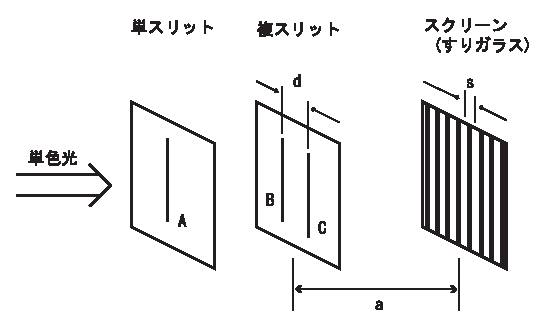
\includegraphics[clip,width=7cm]{1999phys3-1.eps}\\
図1
\end{center}
\begin{center}
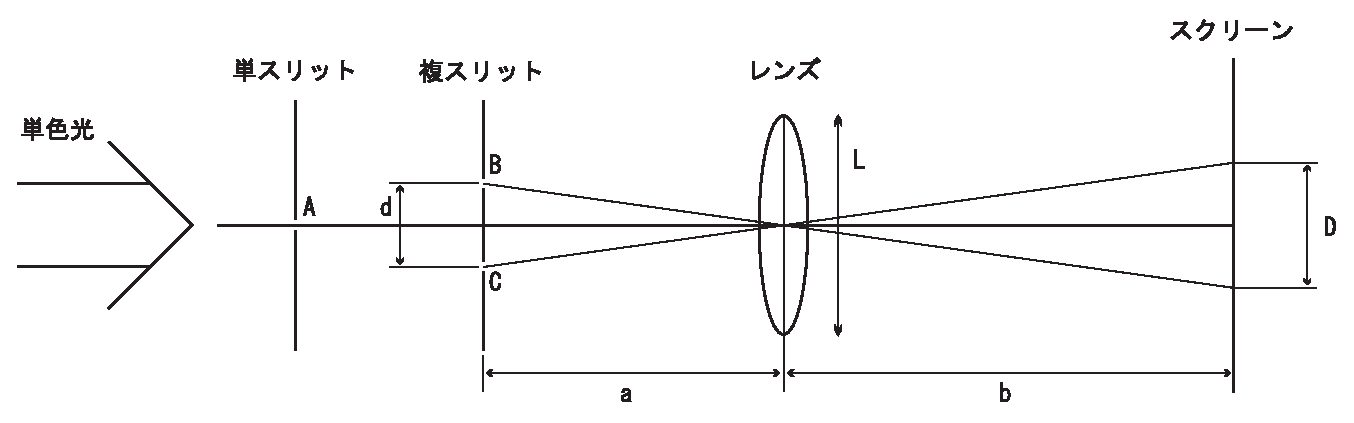
\includegraphics[clip,width=14cm]{1999phys3-2.eps}\\
図2
\end{center}

\end{subsubquestions}

\end{subquestions}

\end{question}
\begin{answer}{教育 物理}{}
\begin{subanswers}
%第1問
\SubAnswer
\begin{subsubanswers}
\SubSubAnswer
重力加速度は、次のように表される。($M_{e}$:地球の質量)
\begin{equation}
g=\frac{GM_{e}}{R^2}\eqname{g}
\end{equation}
またエネルギー保存則より、
\begin{equation}
\frac{1}{2}Mv_{\text{esc}}^2-G\frac{MM_e}{R+h}=0\eqname{ene}
\end{equation}
\eqhref{g}, \eqhref{ene}, $R\gg h$より
\begin{align*}
\frac{1}{2}v_{\text{esc}}^2 &= G\frac{M_e}{R} = gR\\
v_{\text{esc}} &= \sqrt{2gR} \simeq 1.1\times 10^4\ \text{[m/s]}
\end{align*}

\SubSubAnswer
時間$dt$に噴射されるガスの質量を$dm$とすると、ガスの受ける力積は鉛直上向きを正とすると$dm=-dM$より
\[
-u\,dm=u\,dM 
\]
よって、ロケットの受ける力積は $-u\,dM$\newline 
したがって、噴射によりロケットが受ける力積は$-u\frac{dM}{dt}$なので
\[
M\frac{dv}{dt}=-u\frac{dM}{dt}-Mg
\]

\SubSubAnswer
運動方程式より
\[
\frac{dv}{dt}=-\frac{u}{M}\frac{dM}{dt}-g
\]
これを積分すれば
\begin{equation}
\Delta v=u\log \frac{M_i}{M_f}-g\Delta t\eqname{del_u}
\end{equation}
$\Delta v$を大きくするには
\begin{itemize}
\item 噴射速度$u$を大きくする
\item $M_i/M_f$を大きくする(燃料の量を増やす)
\end{itemize}

\SubSubAnswer
$\frac{dv}{dt}=ng$より
\begin{align*}
v &= ng(t-t_0)+v(t_0) \\
h &= \frac{1}{2}ng(t-t_0)^2+v(t_0)(t-t_0)+h(t_0) 
\end{align*}
よって、
\[
\Delta v=ng\Delta t
\]
これを\eqhref{del_u}に代入して
\[
(1+n)g\Delta t=u\log \frac{M_i}{M_f}
\]
ゆえに
\begin{align*}
\Delta t &= \frac{1}{1+n}\frac{u}{g}\log\frac{M_i}{M_f} \\
\Delta v &= \frac{n}{1+n}u\log\frac{M_i}{M_f} \\
\Delta h &= \frac{1}{2}\frac{n}{(1+n)^2}\frac{u^2}{g}\left(\log\frac{M_i}{M_f}\right)^2+v(t_0)\frac{1}{1+n}\frac{u}{g}\log\frac{M_i}{M_f}
\end{align*}

\SubSubAnswer
エネルギー等分配則より、分子の内部構造の自由度を$f$とすると、(たとえば2原子分子なら $f=2$)
\[
\frac{1}{2}mu_0^2=\frac{3+f}{2}kT
\]
よって
\[
u_0=\sqrt{\frac{3+f}{m}kT}
\]
噴射速度を大きくするには、燃料の分子の質量を小さくするか、$f$が大きいものを選べばよい。最良の燃料は水素。

\SubSubAnswer\footnote{より現実的には、液体水素と液体酸素を反応させてできた水分子を噴射することになるので、分子量18$m_p$、$f=6$を用いなければならない、との指摘がある。問題文では燃料として蓄えられた物質の分子量=噴射する分子の分子量となっているように読めるので、そこまで求められているかはわからない。(2003年度注)}
$m\simeq 2m_p=3.4\times 10^{-27}\ $[kg]
\[
u_0=\sqrt{\frac{5\times 1.4\times 10^{-23}\times 2000}{3.4\times 10^{-27}}}=6.4\times 10^3\ \text{[m/s]}
\]

\SubSubAnswer
$v(t_0)=0$とすると
\[
v_f=\frac{4}{5}\times 3\times 10^3\times 2\times 0.7=3.4\times 10^3\ \text{[m/s]}
\]
これは$v_{\text{esc}}$よりもかなり小さい。$v_{\text{esc}}$を得るには、$u$を上げる、つまり、燃焼温度を上げる必要がある。
これには、水素と、それを燃やすのに必要な酸素の混合比を変える方法がある。

混合比の変更のみで十分な温度が得られるか確実でなく、限界があるようであれば、ロケットの一部を逆方向に運動量を与えて切り離すなどの方法を組み合わせる必要が生じる。
\end{subsubanswers}

%第2問
\SubAnswer
\begin{subsubanswers}

\SubSubAnswer
$ j=\rho_-v $

\SubSubAnswer

\parbox[t]{.5\linewidth}{
アンペールの法則より
\begin{enumerate}
\item[(i)]
~$r \leq a$の時
\begin{align*}
2\pi rB&=\mu_0j\pi r^2 \\
B&=\frac{\mu_0j}{2}r
\end{align*}

\item[(ii)]
~$r \geq a$の時
\begin{align*}
2\pi rB&=\mu_0j\pi a^2 \\
B&=\frac{\mu_0ja^2}{2r}
\end{align*}
\end{enumerate}
}
\parbox[t]{.5\linewidth}{
\begin{center}
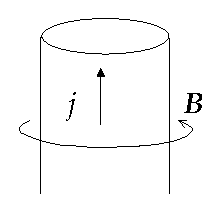
\includegraphics[clip]{1999phys2-1.eps}
\end{center}
}

\SubSubAnswer
\parbox[t]{.5\linewidth}{
\[ F_{\text{Lorentz}}=evB \ (中心内向き)\]
}
\parbox[t]{.5\linewidth}{
\begin{center}
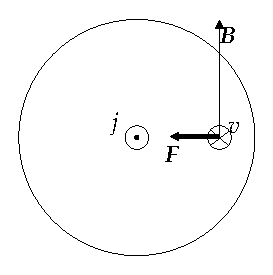
\includegraphics[clip]{1999phys2-2.eps}
\end{center}
}


\SubSubAnswer
\parbox[t]{.5\linewidth}{
ガウスの法則より($E$は外向きを正とする)
\begin{align*}
2\pi rlE&=\frac{1}{\eps _0}(\rho_0-\rho_-)l\pi r^2 \\
E&=\frac{\rho_0-\rho_-}{2\eps _0}r \; (中心内向き)
\end{align*}
}
\parbox[t]{.5\linewidth}{
\begin{center}
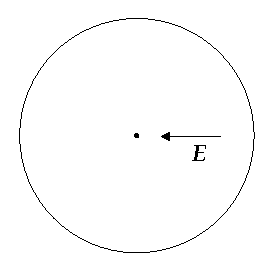
\includegraphics[clip]{1999phys2-3.eps}
\end{center}
}

\SubSubAnswer
負電荷が多く分布する。

\SubSubAnswer
$ \rho_+=\rho_-$より$\Delta \rho_+=0$.また、
$ \Vec{F}_{\text{Lorentz}}+(-e)\Vec{E}=0$より
\begin{align*}
ev\: \frac{\mu_0\rho_-v}{2}r&=e\: \frac{\rho_--\rho_0}{2\varepsilon_0}r \\
\frac{v^2}{c^2}\rho_-&=\rho_--\rho_0 \qquad \left(  c^2=\frac{1}{\mu_0 \eps_0}\right) \\
\therefore -\rho_- &=-\frac{\rho_0}{1-v^2/c^2} \\
	&\simeq -\left( 1+\frac{v^2}{c^2} \right) \rho_0 \\
\end{align*}
\[ \therefore \Delta(-\rho_-)=-\frac{v^2}{c^2}\rho_0 \]

\SubSubAnswer
電子の数密度を$n$とすると
\begin{gather*}
n=\frac{9\times10^3~\mathrm{[kg\cdot m^{-3}]}\cdot6\times10^{23}~\mathrm{[mol^{-1}]}}{63.55\times10^{-3}~\mathrm{[kg\cdot mol^{-1}]}}\fallingdotseq 8.4\times10^{28}~\mathrm{[m^{-3}]} \\
\rho_-=1.6\times10^{-19}~\mathrm{[C]}\cdot8.4\times10^{28}~\mathrm{[m^{-3}]}\fallingdotseq 1.3\times10^{10}~\mathrm{[C\cdot m^{-3}]} \\
j=\frac{1~\mathrm{[A]}}{10^{-6}~\mathrm{[m^2]}}=10^6~\mathrm{[A\cdot m^{-2}]} \\
\therefore v=\frac{j}{\rho_-}\fallingdotseq 7.6\times10^{-5}~\mathrm{[m/s]}\fallingdotseq 8\times10^{-5}~\mathrm{[m/s]}\\
\therefore \frac{\Delta \rho_-}{-\rho_0}=\left(\frac{v}{c}\right)^2\fallingdotseq 6\times10^{-26}
\end{gather*}

\end{subsubanswers}

%第3問
\SubAnswer
\begin{subsubanswers}
\SubSubAnswer
\parbox[t]{.5\linewidth}{
\begin{align*}
d\sin\theta&=m\lambda\\
\frac{dy}{a}&=m\lambda
\end{align*}
\[ \therefore s=\frac{a}{d}\lambda=1\times10^{-3}\mathrm{m} =1\mathrm{mm}\]
}
\parbox[t]{.5\linewidth}{
\begin{center}
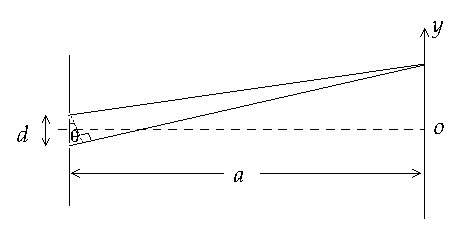
\includegraphics[clip]{1999phys3-3.eps}
\end{center}
}

\SubSubAnswer
$ 公式 \: \dfrac{1}{a}+\dfrac{1}{b}=\dfrac{1}{f} \:$より
\begin{gather*}
b=\frac{af}{a-f}=45\mathrm{cm} \\
D=\frac{b}{a}d=\frac{45}{5}\cdot 30\mathrm{\mu m}=0.27\mathrm{mm} \\
\end{gather*}

\SubSubAnswer
$d=2\mathrm{\mu m}$より$s=15\mathrm{mm}$。一方、レンズの半径は10mm。\\
よって、レンズには0次回折光の情報しか来ていないのでスリットが単スリットである時と同じ状況になっている。だから、スクリーンにはまるで単スリットから出た光のような像がうつる。

\SubSubAnswer
1次回折光がレンズを通ればよい。レンズの半径は1cmだから
\[ d_0=\frac{5\mathrm{cm}\times0.6\mathrm{\mu m}}{1\mathrm{cm}}=3\mathrm{\mu m} \]

\SubSubAnswer
\begin{itemize}
\item[(i)]
波長を変えない時 \\
レンズを大きくする。\\
半径1.5cm以上にすれば1次回折光がレンズを通るから。
\item[(ii)]
 波長を変える時 \\
波長を短くする。\\
$s$が小さくなって1次回折光がレンズを通るから。
\end{itemize}
\end{subsubanswers}

\end{subanswers}
\end{answer}



\end{document}
